
\newpage

\chapter{Toward Congruence and Similarity}
Need to renumber so the section number is correct. 

\section{Similar Triangles}

One day when aloof old Professor Rufus was trying to explain similar
triangles to his class, he merely wrote
\[
\tri ABC \sim \tri A'B'C' \qquad\Leftrightarrow \qquad\begin{array}{l}
\angle A \simeq \angle A'\\
\angle B \simeq \angle B' \\
\angle C \simeq \angle C'
\end{array}
\]
and walked out of the room.

\begin{question} 
Can you give $3$ much needed examples of similar triangles? 
\end{question}
\QM

\begin{question} 
Devise a way to use folding and tracing constructions to help explore this notion
of similar triangles.
\end{question}
\QM

Another day when aloof old Professor Rufus was trying to explain
similar triangles to his class, he merely wrote
\[
\tri ABC \sim \tri A'B'C' \qquad\Leftrightarrow \qquad
\begin{array}{l}
AB = k\cdot A'B'\\
BC = k\cdot B'C' \\
CA = k\cdot C'A'
\end{array}
\]
and walked out of the room.

\begin{question} 
Can you give $3$ much needed examples of similar triangles? 
\end{question}
\QM

\begin{question} 
Devise a way to use folding and tracing constructions to help explore this notion
of similar triangles.
\end{question}
\QM



\begin{question} 
What's going on in aloof old Professor Rufus' head?  (I realize that
this is a dangerous question!)  Why are his explanations so different?
\end{question}
\QM


%%%%%%%%%%%%%%%%%%%%%%%%%%%%%%%%%%%%%%%%%%%
%% UPSHOT: Either defintion is good for this course. There
%% will/should-be handouts proving AA and SSS for similarity, hence
%% proving they are the same.
%%%%%%%%%%%%%%%%%%%%%%%%%%%%%%%%%%%%%%%%%%%



\subsection{Theorems for Similar Triangles}

In this section we will show that that \textbf{both} definitions of similar
triangles given above are \textbf{equivalent}.  We'll start with a gentle
question:

\begin{question} What is the formula for the area of a triangle?
\end{question}
\QM

Using merely the formula for the area of a triangle, we (meaning you)
will explain why the following important theorem is true. Throughout this 
discussion we will use the convention that when we
write $AB$ we mean the \textit{length} of the segment $AB$.


\begin{theorem}[Parallel-Side] 
\index{Parallel-Side Theorem}\index{Theorem!Parallel-Side}
Given:
\[
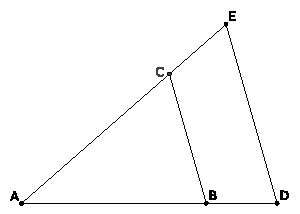
\includegraphics{../graphics/split1.pdf}
\]
If side $BC$ is parallel to side $DE$, then
\[
\frac{AB}{AD} = \frac{AC}{AE}.
\] 
\end{theorem}

\begin{question}
Can you tell me in English what this theorem says? Provide some
examples of this theorem in action.
\end{question}
\QM

Now we (meaning you) are going to explore a bit. See if answering
these questions sheds light on this.

\begin{question} 
If $h$ is the height of $\tri ABC$, find a formula for the areas of
$\tri ABC$ and $\tri ADC$.
\[
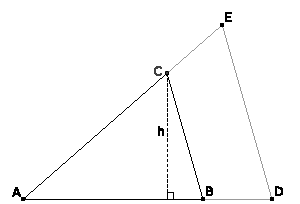
\includegraphics{../graphics/split2.pdf} \qquad 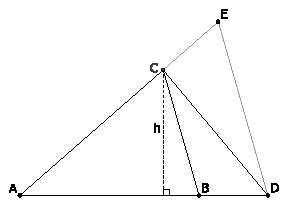
\includegraphics{../graphics/split3.pdf}
\]
\end{question}
\QM

\begin{question} 
If $g$ is the height of $\tri ACB$, find a formula for the areas of
$\tri ACB$ and $\tri AEB$.
\[
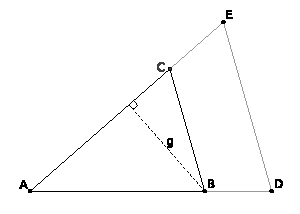
\includegraphics{../graphics/split4.pdf} \qquad 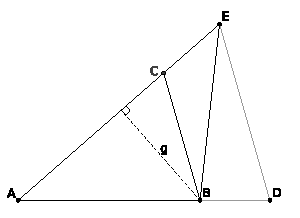
\includegraphics{../graphics/split5.pdf}
\]
\end{question}
\QM


\begin{question} Explain why 
\[
\mathrm{Area}(\tri ABC) = \mathrm{Area}(\tri ACB).
\]
\end{question}
\QM

\begin{question} Explain why 
\[
\mathrm{Area}(\tri CBE) = \mathrm{Area}(\tri CBD).
\]
Big hint: Use the fact that you have two parallel sides! Draw a
picture to help clarify your explanation.
\end{question}
\QM

\begin{question} Explain why 
\[
\mathrm{Area}(\tri ADC)= \mathrm{Area}(\tri AEB).
\]
\end{question}
\QM

\begin{question}
Explain why
\[
\frac{\mathrm{Area}(\tri ABC)}{\mathrm{Area}(\tri ADC)} = \frac{ \mathrm{Area}(\tri ACB)}{\mathrm{Area}(\tri AEB)}
\]
\end{question}
\QM

\begin{question} Compute and simplify both of the following expressions:
\[
\frac{\mathrm{Area}(\tri ABC)}{\mathrm{Area}(\tri ADC)} \qquad\text{and}\qquad\frac{ \mathrm{Area}(\tri ACB)}{\mathrm{Area}(\tri AEB)}
\]
\end{question}
\QM


\begin{question} How can you conclude that: 
\[
\frac{AB}{AD} = \frac{AC}{AE}
\]
\end{question}
\QM

\begin{question} 
Why is it important that line $DE$ is parallel to line $CB$?
\end{question}
\QM


\begin{question} 
Can you sketch out (in words) how the questions above prove the Parallel-Side
Theorem?
\end{question}
\QM

Now comes the moment of truth. 
\begin{question}
Can you use the Parallel-Side Theorem to explain why if you know that
if you have two triangles, $\tri ABC$ and $\tri A'B'C'$ with:
\begin{align*}
\angle A &\simeq \angle A'\\
\angle B &\simeq \angle B' \\
\angle C &\simeq \angle C'
\end{align*}
then we must have that
\begin{align*}
AB &= k\cdot A'B'\\
BC &= k\cdot B'C'\\
CA &= k\cdot C'A'
\end{align*}
\end{question}
\QM






\subsubsection{The Converse}

The converse of the Parallel-Side Theorem states:

\begin{theorem}[Split-Side]\index{Split-Side Theorem}\index{Theorem!Split-Side} 
Given:
\[
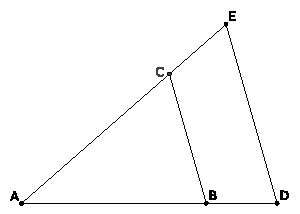
\includegraphics{../graphics/split1.pdf}
\]
If side $BC$ intersects (splits) the sides of $\tri ADE$ so that
\[
\frac{AB}{AD} = \frac{AC}{AE},
\] 
then side $BC$ is parallel to side $DE$.
\end{theorem}

\begin{question} 
How could you investigate this theorem using any of the construction
techniques above?
\end{question}
\QM

Now we (meaning you) will answer questions in the hope that they will
help us see why the above theorem is true.

\begin{question}
Suppose that you \textbf{doubt} that side $BC$ is parallel to side $DE$. Explain
how to place a point $C'$ on side $AE$ so that side $BC'$ is
parallel to line $DE$. Be sure to sketch the situation(s).
\end{question}
\QM

\begin{question} 
You now have a triangle $\tri ADE$ whose sides are split by a line
$BC'$ such that the line $BC'$ is parallel to line $DE$. What does the
Parallel-Side Theorem have to say about this?
\end{question}
\QM

\begin{question} What can you conclude about points $C$ and $C'$?
\end{question}
\QM


\begin{question} 
What does this tell you about the Split-Side Theorem?
\end{question}
\QM




Let's see if you can put this all together:
\begin{question}
Can you use the Split-Side Theorem to explain why if you know that
if you have two triangles, $\tri ABC$ and $\tri A'B'C'$ with:
\begin{align*}
AB &= k\cdot A'B'\\
BC &= k\cdot B'C'\\
CA &= k\cdot C'A'
\end{align*}
then we must have that
\begin{align*}
\angle A &\simeq \angle A'\\
\angle B &\simeq \angle B' \\
\angle C &\simeq \angle C'
\end{align*}
\end{question}
\QM

Putting all of our work above together, we may now say the following:





\begin{definition}\index{similar triangles} 
Two triangles $\tri ABC$ and $\tri A'B'C'$ are said to be
\textbf{similar} if either equilvalent condition holds:
\[
\begin{array}{l}
\angle A \simeq \angle A'\\
\angle B \simeq \angle B' \\
\angle C \simeq \angle C'
\end{array}
\qquad\text{or}\qquad
\begin{array}{l}
AB = k\cdot A'B'\\
BC = k\cdot B'C' \\
CA = k\cdot C'A'
\end{array}
\]
\end{definition}



\subsubsection{SAS-Similarity Theorem}







\begin{theorem}[SAS-Similarity Theorem]
\index{Theorem!SAS Similarity}\index{SAS-Similarity Theorem} Knowing
the ratio of the lengths of two sides and the measure of the angle
between them, determines a triangle up to similarity. In pictures, we have something like:
\[
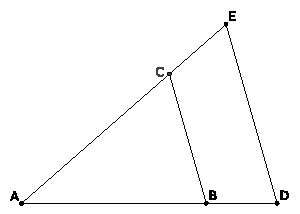
\includegraphics{../graphics/split1.pdf}
\]
\[
\frac{AB}{AC} = \frac{AD}{AE} \qquad\Rightarrow\qquad \tri ABC \simeq \tri ADE.
\]
\end{theorem}

\begin{question} What does this mean, ``up to similarity?''
\end{question}
\QM

Let's see if we (meaning you) can get to the bottom of why this
theorem is true. This time, you're going to produce the
illustrations. Use folding and tracing why not!

\begin{question}
Fold any triangle. Now fold another triangle sharing one of the angles
so that the ratio of the lengths of the sides are the same in both
triangles. The sides touching the angle should share folds. You should
see some parallel lines. Which theorem above says that this should
happen?
\end{question}
\QM

\begin{question} 
What do we know about parallel lines crossing another line?
\end{question}
\QM

\begin{question} 
Can you sketch out (in words) how the questions above prove the SAS-Similarity
Theorem?
\end{question}
\QM


\subsection{A Meaning of Multiplication}

Do you ever sit around asking yourself what different things
\textit{mean}? For example, ``What does being happy really mean?'' In
mathematics we don't dare try to tackle a brain-buster like that
one. Instead we try to focus on simple problems.

\begin{question} What can multiplication mean? 
\end{question}
\QM

I have no idea how you might have answered that question. Anyhow,
maybe you can answer the next questions:

\begin{question} 
Can you give multiplication meaning involving groups of groups or
something of the sort?
\end{question}
\QM

\begin{question} 
Can you give multiplication meaning involving areas or something of
the sort?
\end{question}
\QM

\begin{question}
Compare and contrast the two meanings of multiplication given above.
\end{question}

OK---all of this is fine and good, but we one little problem. If
numbers by themselves ``mean'' lengths and numbers multiplied together
``mean'' areas, how do we do something like this:
\[
\underbrace{3}_\text{length} + \underbrace{4\cdot 5}_\text{area}?
\]


I say we can use similar triangles to save the day!


\begin{question} 
Can you somehow give ``meaning'' to multiplication using similar
triangles? Hint: One of them should have a side of length $1$.
\end{question}
\QM

